\chapter{Faults in Flow-Based Biochips}
\label{chap:faults}
This chapter will outline the possible faults and their causes in flow-based biochips. Furthermore, it will outline the fault-modeling of the defects and describe the recently developed automated testing technique for flow-based biochips.

\section{Possible Faults and Causes}
Defects in a flow-based microfluidic biochip can be attributed to fabrication steps and environmental reasons such as imperfections in molds, pollutants, bubbles in PDMS gel, and failure in hard baking. Furthermore, as feature sizes are scaled down, the sizes of and distances between microchannels are reduced in order to achieve higher degrees of microfluidic integration. This increasing density raises the likelihood of defects \cite{fault-modeling}. Some typical defects are listed below.

\begin{figure}
\centering
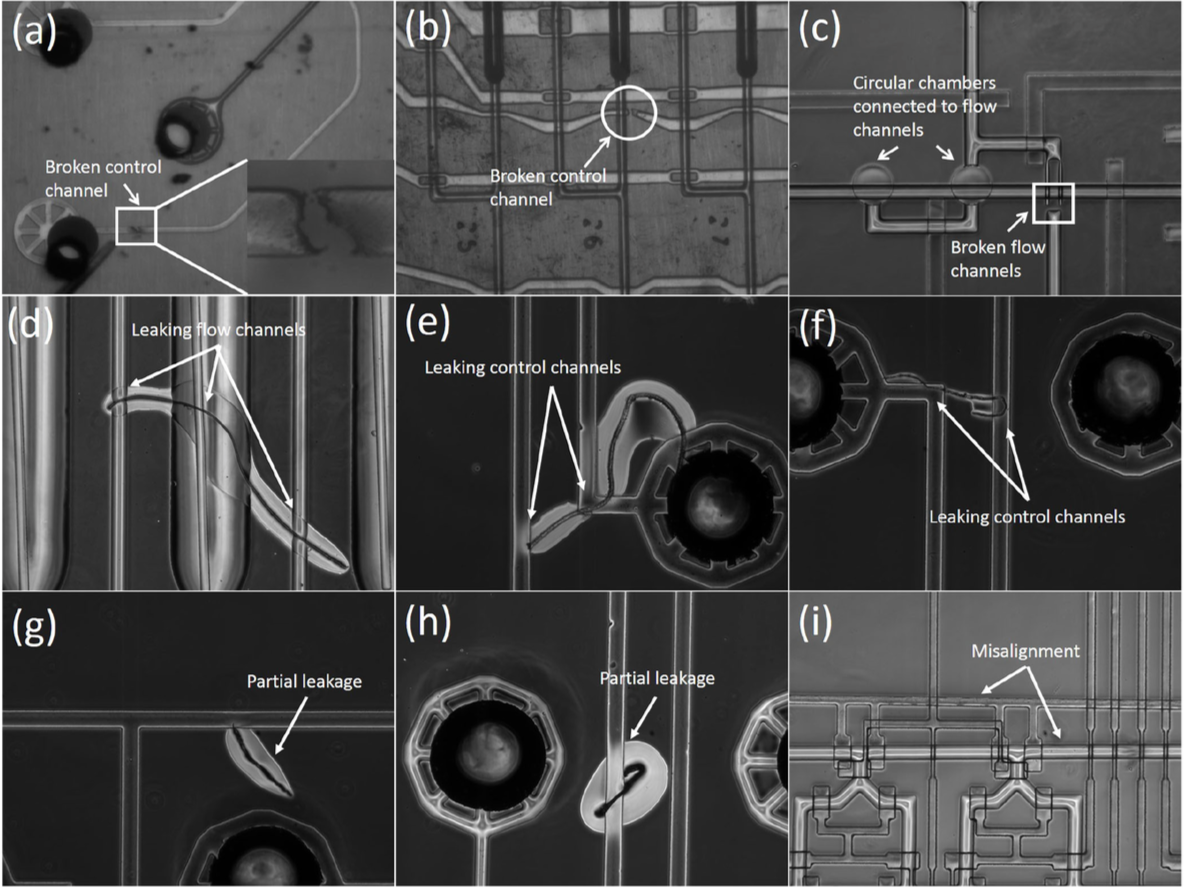
\includegraphics[scale=0.45]{figures/possible-faults.png}
\caption[Possible faults in flow-based biochips]{Possible faults in flow-based biochips \cite{fault-modeling}.}
\label{fig:possible-faults}
\end{figure}

\begin{itemize}
\item \emph{Block:} Channels may be disconnected, blocked or even missing. \autoref{fig:possible-faults}(a)-(c) show some examples of the block defect in fabricated microfluidic biochips. The possible causes for block defects are environmental particles or imperfection in silicon wafer mold.

\item \emph{Leak:} It is possible that some defective spots on the wall can connect independent channels. Thereby the flows in either of the channels infiltrate the other channel, which will result in a cross-contamination that can be catastrophic. The probability of  a leaked channel pair increases as the length of the channels increases. Additionally the probability becomes greater if the distance between parallel channels decreases, and similarly the probability is smaller for channels that do not run in parallel. \autoref{fig:possible-faults}(d)-(f) shows some examples of leak defects that are caused by fiber pollutant in fabricated microfluidic biochips. Some partial leak defects are shown in \autoref{fig:possible-faults}(g) and \autoref{fig:possible-faults}(h). These defective spots may become full leakage when high pressure is injected into the channels.

\item \emph{Misalignment:} The control layer and the flow layer of the biochip are misaligned. \autoref{fig:possible-faults}(i) shows the defect. The result of this is that membrane valves either cannot be closed or are not even formed.

\item \emph{Faulty Pumps:} Pumps with defects fail to generate pressure when actuated. The transmission of pressure is interrupted.

\item \emph{Degradation of Valves:} The membranes of valves may lose their flexibilities or they might even be perforated after a large number of operations. The result is that the valves cannot seal flow channels.

\item \emph{Dimensional Errors:} The actual fabricated microfluidic biochip might be too narrow compared to the designed dimensions. The mismatch of height-to-width ratio may lead to a valve that cannot be closed.

\end{itemize}

\section{Defects and Fault Modeling}
Despite the complexity of flow-based biochips the consequences of the defects can be described as either a block or a leak \cite{fault-modeling}. These two generic faults (block and leak) can be observed in both the control layer and the flow layer, however their respective faulty behaviours are different. Their faulty behaviours are described in \autoref{tab:faulty-behaviour}. Therefore we can describe the possible defects in a flow-based biochip and their respective fault model, which is given in \autoref{tab:defect-fault-model}.

\begin{table}[H]
\centering
\caption{Defects and fault modeling}
\begin{tabular}{| c | c | c | c |}
\hline
\textbf{Defect} & \textbf{Fault model}\\ \hline
Block & Block in control/flow channel\\ \hline
Leak / partial leak & Leak in control/flow channel\\ \hline
Misalignment between flow and control layer & Block in control channel\\ \hline
Faulty pumps & Block in control/flow channel\\ \hline
Degradation of valves & Block in control channel\\ \hline
Dimensional errors & Block in control channel\\ \hline
\end{tabular}
\label{tab:defect-fault-model}
\end{table}

Misalignment between flow and control layer can be modeled as the faulty behaviour of block in the control channels. This is possible as the result of the defect is that membrane valves either cannot be closed or are not even formed \cite{fault-modeling}.
The behaviour of faulty pumps is similar to the faulty behaviour of a block as the transmission of pressure is interrupted \cite{fault-modeling}.
Degradation of valves can be modeled as a block in a control channel as the valves cannot seal flow channels \cite{fault-modeling}.
Dimensional errors have similar faulty behaviour as that of a block in a control channel as a valve cannot be closed, i.e. the flow cannot be stopped in flow channels underneath the valve \cite{fault-modeling}.\\

\begin{table}[H]
\centering
\caption{Faulty behaviour of block and leak \cite{fault-modeling}}
\begin{tabular}{| c | >{\centering\arraybackslash} m{4.8cm} | >{\centering\arraybackslash} m{4.8cm} |}
\hline
${}$ & \textbf{Flow Layer} & \textbf{Control Layer}\\ \hline
Block & Fluid flow cannot go through the obstacle inside the channel so transport is blocked. & Pressure cannot reach the flexible membrane, which prevents the corresponding valve from closing. \\ \hline
Leak & Fluid flow permeates the adjacent microchannels. & Control channels of two independent valves are unintentionally connected. Pressure on either valve activates both. \\ \hline
\end{tabular}
\label{tab:faulty-behaviour}
\end{table}

\section{Fault Model}
The errors due to defects can be modeled in terms of faulty behaviours of valves \cite{fault-modeling}. For example a block in a flow channel can be modeled as a valve that cannot be opened, i.e. the valve cannot be deactivated. While a block in a control channel can be modeled as a valve that cannot be closed, i.e. the valve cannot be activated. Similar behaviour models can be defined for leaks.

\begin{figure}[H]
\centering
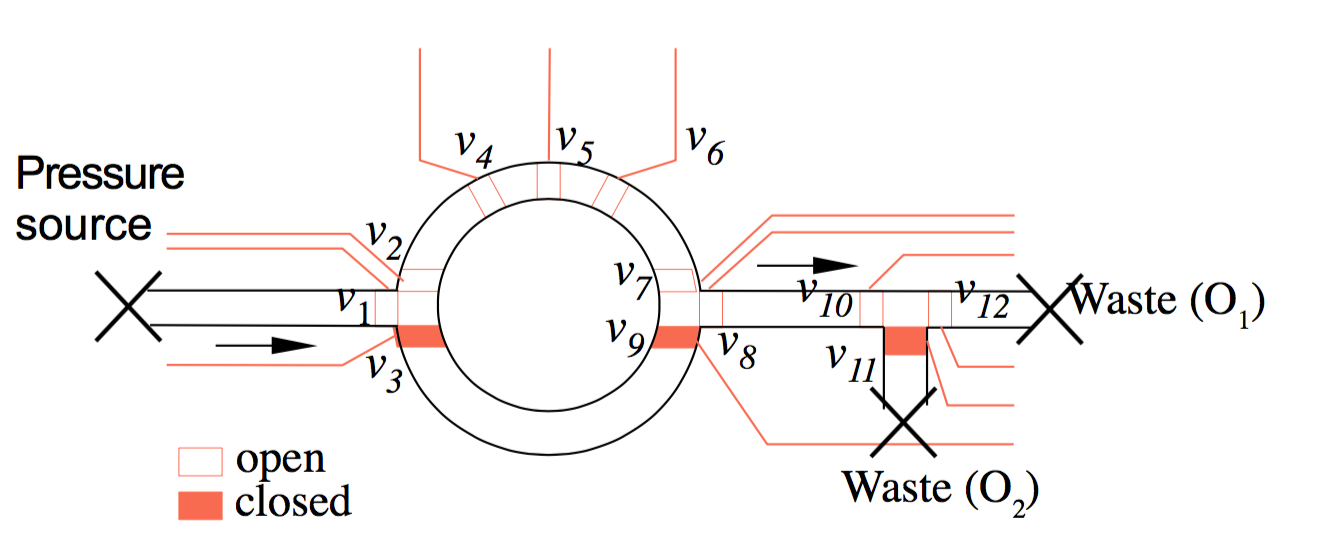
\includegraphics[scale=0.4]{figures/fault-model-example.png}
\caption[Simple microfluidic biochip]{Simple microfluidic biochip}
\label{fig:fault-model-example}
\end{figure}

\autoref{fig:fault-model-example} shows a layout of a simple microfluidic biochip with a mixer. The rectangles indicate positions of valves and the black lines indicate flow channels. Consider \autoref{fig:fault-model-example} and consider the following defects.
\begin{itemize}
\item \emph{Block in flow channel}: A block defect in the flow channel between valves $v_3$ and $v_9$ leads to the behaviour that valve $v_3$ cannot be opened. A valve and the channels connected to it are considered to be a single entity.

\item \emph{Leak in flow channel}: If a leak occurs between the flow channels $v_3$-$v_9$ and $v_2$-$v_4$, the liquid in channel $v_3$-$v_9$ infiltrates channel $v_2$-$v_4$

\item \emph{Block in control channel}: If a block occurs in a control channel then pressurised air cannot reach the flexible membrane to seal the flow channel. In this case valve $v_9$ cannot be closed.

\item \emph{Leak in control channel}: If a leak occurs between the control channels of $v_4$ and $v_9$, the two shorted valves effectively form one valve. The result is that whenever either valve is activated then both valves are activated, i.e. whenever $v_4$ is closed then $v_9$ is also closed.

\end{itemize}

\section{Fault-Specific Testing Strategy}
We use the testing strategy for flow-based biochips as proposed in \cite{fault-modeling}. The used test set up has feedback generated when pressure sensors are connected to the outlets and pumps are connected to the inlets. If a path exists between the pump sources (inlets) and pressure sensors (outlets), pressure sensors at the outlets will detect a high pressure generated by the pumps. The measured high pressure is defined as output "1". If all paths between inlets and outlets are blocked, pressure sensors cannot sense the high pressure injected by the pumps. This is defined as output "0". All ports in flow-based biochips are identical, regardless of functional classification. When testing, only one of the ports in the flow layer is connected to a pressure source and the rest to pressure sensors. \\
Consequently the definitions for valve conditions can be formulated. \autoref{tab:valve-logic} connects the logic representation of valve states to the corresponding pressure response.

\begin{table}[H]
\centering
\caption{Logic representation of valve states and pressure response \cite{fault-modeling}}
\begin{tabular}{| c | c | c | c |}
\hline
\textbf{Logic} & \textbf{Valve state} & \textbf{Valve condition} & \textbf{Pressure response}\\ \hline
1 & open & deactivated & high\\ \hline
0 & closed & activated & low \\ \hline
\end{tabular}
\label{tab:valve-logic}
\end{table}

A binary pattern (test vector) is applied to all valves to set their/open close states. The actual responses of pressure sensors are compared to the expected responses. If these two sets match then the biochip is considered good.\\

\autoref{tab:testing-strategy} shows the testing strategy to target the faults in \autoref{tab:faulty-behaviour}. The test effectiveness is dependent on the quality of the test patterns. The more complicated the biochip structure is, the harder it is to determine a test pattern set that covers every fault type for each valve and channel.

\begin{table}[H]
\centering
\caption{Testing strategy for different kinds of faults \cite{fault-modeling}}
\begin{tabular}{| c | >{\centering\arraybackslash} m{4.8cm} | >{\centering\arraybackslash} m{4.8cm} |}
\hline
${}$ & \textbf{Flow Layer} & \textbf{Control Layer}\\ \hline
Block & Position: $v_3$-$v_9$. Both valves $v_3$ and $v_9$ are deactivated to form a route $inlet$-$v_1$-$v_3$-$v_9$-$v_8$-$v_{10}$-$v_{11}$-$O_2$. If the output at $O_2$ is "0", the defect is detected. & Position: valve $v_9$. The block in the control layer prevents valve from closing. Deactivate valve $v_1$, $v_3$, $v_8$, $v_{10}$, $v_{11}$ and $O_2$ but activate the rest including $v_9$. If $O_2$ is "1" the defect is detected. \\ \hline
Leak & Position between $v_3$-$v_9$ \& $v_2$-$v_4$. Deactivate valve $v_1$, $v_2$, $v_9$, $v_8$, $v_{10}$ and $v_{11}$. If high pressure is sensed at $O_2$, the leaking defect is detected. & Position: $v_7$ \& $v_9$. Turn on valve $v_1$, $v_3$, $v_9$, $v_8$, $v_{10}$ and $v_{11}$ but activate $v_7$. If there is a leakage, high pressure in control channel $v_7$ will activate $v_9$ and block the route.\\ \hline
\end{tabular}
\label{tab:testing-strategy}
\end{table}

Due to the difficulty of determining a test pattern set the more complicated a biochip structure is, there is a need to further abstract faults and microfluidic structures to facilitate automatic test-vector generation.

\section{General Testing Strategy}
\label{sec:general-testing-strategy}
\autoref{tab:behaviour-level} defines the behavioural-level fault models for a flow-based biochip. This definition is possible since the defects can be modeled as faulty behaviour of a valve and a binary logic framework can be defined where an activated valve can be defined as "0" and a deactivated valve as "1".

\begin{table}[H]
\centering
\caption{Behavioural-level fault model for flow-based biochips \cite{fault-modeling}}
\begin{tabular}{| c | c | c | c |}
\hline
${}$ & \textbf{Flow Layer} & \textbf{Control Layer} \\ \hline
Block & stuck-at-0 & stuck-at-1 \\ \hline
Leak & OR-bridge (1-dominant) & AND bridge (0-dominant) \\ \hline
\end{tabular}
\label{tab:behaviour-level}
\end{table}

All types of defects in control and flow channels can be mapped to specific behaviour-level fault at a valve. By virtue of this classification the testing problem is simplified from a 3-D structure to that of a 2-D design. Biochips with complicated networks of channels and valves have their test generation simplified because of this.


\begin{figure}[H]
\centering
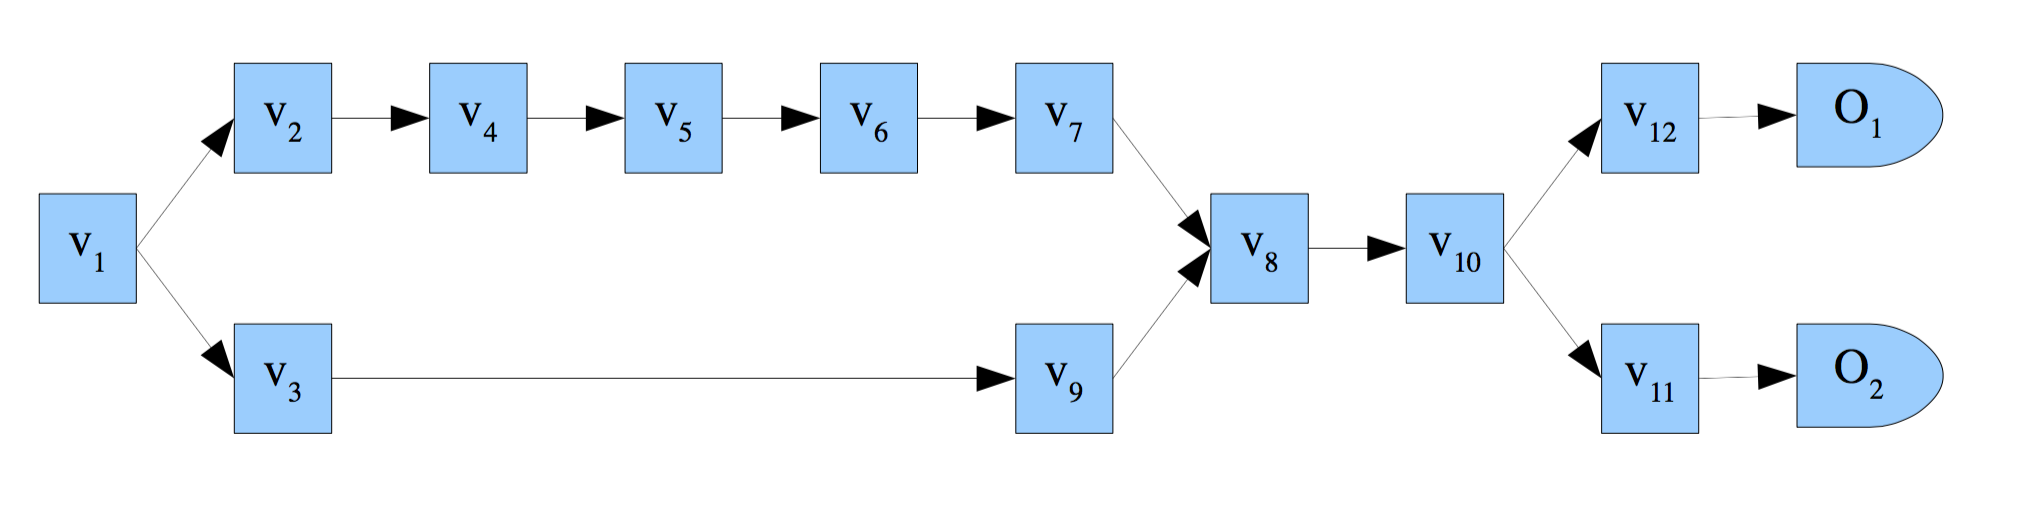
\includegraphics[scale=0.35]{figures/valve-network.png}
\caption[Schematic of a valve network corresponding to \autoref{fig:fault-model-example}. Adapted from \cite{fault-modeling}]{Schematic of a valve network corresponding to \autoref{fig:fault-model-example}. Adapted from \cite{fault-modeling}}
\label{fig:valve-network}
\end{figure}

In order to easily describe and analyse biochip channel networks, a discretised schematic is developed in \cite{fault-modeling} in place of a continuos fluid-flow topology. \autoref{fig:valve-network} illustrates the design by using the biochip design in \autoref{fig:fault-model-example}. This schematic infers logic relationships that define flow-based biochips. \autoref{fig:valve-network} infers that valve $v_2$ is serially connected to valve $v_4$, $v_5$, $v_6$, and $v_7$. Hence either valve can potentially block the route, i.e. there is an "AND" logic relationship among the valves. Contrary routes $v_2$-$v_7$ and $v_3$-$v_9$ are in parallel. Therefore the activation of either of the two routes can lead to output "1". There is an "OR" logic relationship between them.

The flow-based biochips can be further abstracted from the schematic representative of valve networks to valve-based logic gate circuit diagrams \cite{fault-modeling}. This is shown in \autoref{fig:logic-circuit-model} using \autoref{fig:fault-model-example} as an example.

\begin{figure}
\centering
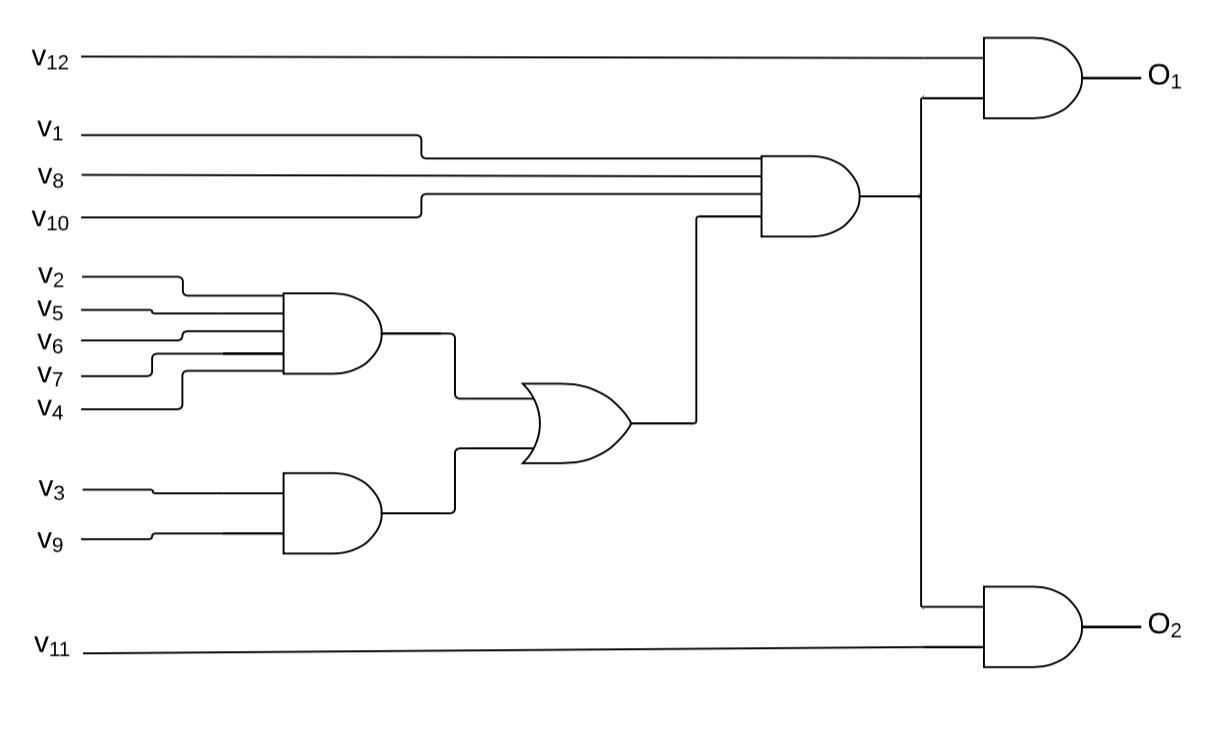
\includegraphics[scale=0.55]{figures/logic-circuit-model.png}
\caption[Logic circuit model of the biochip in \autoref{fig:fault-model-example}. Adapted from \cite{fault-modeling}]{Logic circuit model of the biochip in \autoref{fig:fault-model-example}. Adapted from \cite{fault-modeling}}
\label{fig:logic-circuit-model}
\end{figure}

The logic expression of \autoref{fig:logic-circuit-model} is $\{O_1, O_2\} = \{v_{11}, v_{12}\} \cdot v_1 \cdot v_8 \cdot v_{10} \cdot (v_2 \cdot v_4 \cdot v_5 \cdot v_6 \cdot v_7 + v_3 \cdot v_9)$. The primary inputs are nodes in the schematic of \autoref{fig:valve-network}. The following is the important attributes of the logic circuit model.

\begin{itemize}
\item Only primary inputs (valves) and outputs (pressure sensors) have physical meaning. All other circuit connections are used to represent logical relationship. By virtue of this, it is only necessary to target faults at the primary inputs of this circuit.
\item A series connection of valves in a flow route is mapped to an AND gate. Contrary a parallel connection of valves is mapped to an OR gate.
\end{itemize}

A physical defect in a flow-based biochip can be mapped to a fault at a primary input of a logic circuit. This is based on \autoref{fig:logic-circuit-model} and \autoref{tab:behaviour-level}. Targeting the block defect in the flow channel $v_3$-$v_9$ is done by mapping the defect to a stuck-at-0 according to \autoref{tab:behaviour-level}. Afterwards, the fault is associated with the primary input $v_3$ in the logic circuit model in \autoref{fig:logic-circuit-model}. A leak defect between valve $v_7$ and $v_9$ can be represented by an AND bridge fault between primary inputs $v_7$ and $v_9$ of \autoref{fig:logic-circuit-model}. As a result of the logic circuit model it is possible to readily determine the actual (with faults) and expected (fault-free) responses of pressure sensors and hence accelerate the search for test stimuli. If the actual output differ from the expected output, it is possible to not only conclude that the biochip is faulty, but also infer the positions and types of defects.

\section{Summary}
In this chapter the possible faults and causes in a flow-based biochip are outlined. The faults and causes can be attributed to fabrication steps and environmental reasons. The consequences of the faults can be modeled as either a block or a leak in flow or control channels. The errors due to defects can be modeled in terms of faulty behaviours of valves. This fact is used to devise an automated testing strategy that uses a logic circuit model to determine if a given biochip is faulty and the types and positions of the defects.